% ==============================================================================
% Projeto de Sistema - Gustavo Steim da Silveira
% Capítulo 5 - FrameWeb
% ==============================================================================
\chapter{Modelagem FrameWeb}
\label{sec-frameweb}
\vspace{-1cm} % Ajuste este espaçamento se necessário

\emph{\imprimirtitulo} é um sistema Web cuja arquitetura utiliza o padrão em camadas, com tecnologias e \textit{frameworks} da plataforma .NET. Embora a abordagem FrameWeb tenha sido originalmente proposta com base em tecnologias Java (como JSF, CDI, JPA e JAAS), seus conceitos podem ser adaptados para outras plataformas, como demonstrado neste capítulo.

A Tabela~\ref{tabela-frameworks} apresenta a correspondência entre os tipos de \textit{frameworks} definidos pela abordagem FrameWeb e os utilizados no presente sistema. Em seguida, são apresentados os modelos FrameWeb para cada camada da arquitetura: Negócio, Acesso a Dados e Apresentação.

\begin{table}[H]
\centering
\caption{\textit{Frameworks} da arquitetura do sistema separados por categoria.}
\label{tabela-frameworks}
\begin{tabular}{|c|c|}
\hline
\textbf{Categoria de \textit{Framework}}& \textbf{\textit{Framework} Utilizado} \\\hline
Controlador Frontal & ASP.NET Core MVC \\\hline
Injeção de Dependências & Microsoft.Extensions.DependencyInjection \\\hline
Mapeamento Objeto/Relacional & Entity Framework Core \\\hline
Segurança & ASP.NET Identity \\\hline
\end{tabular}
\end{table}

\section{Camada de Negócio}
\label{sec-frameweb-negocio}

Nesta camada, o modelo de entidades e o modelo de aplicação foram representados conforme a abordagem FrameWeb. Embora o modelo do FrameWeb não tenha sido originalmente proposto para a plataforma .NET, os conceitos de \textbf{entidades de domínio} e \textbf{serviços de aplicação} foram mapeados diretamente para os componentes do sistema implementado.

\begin{figure}[H]
	\centering
	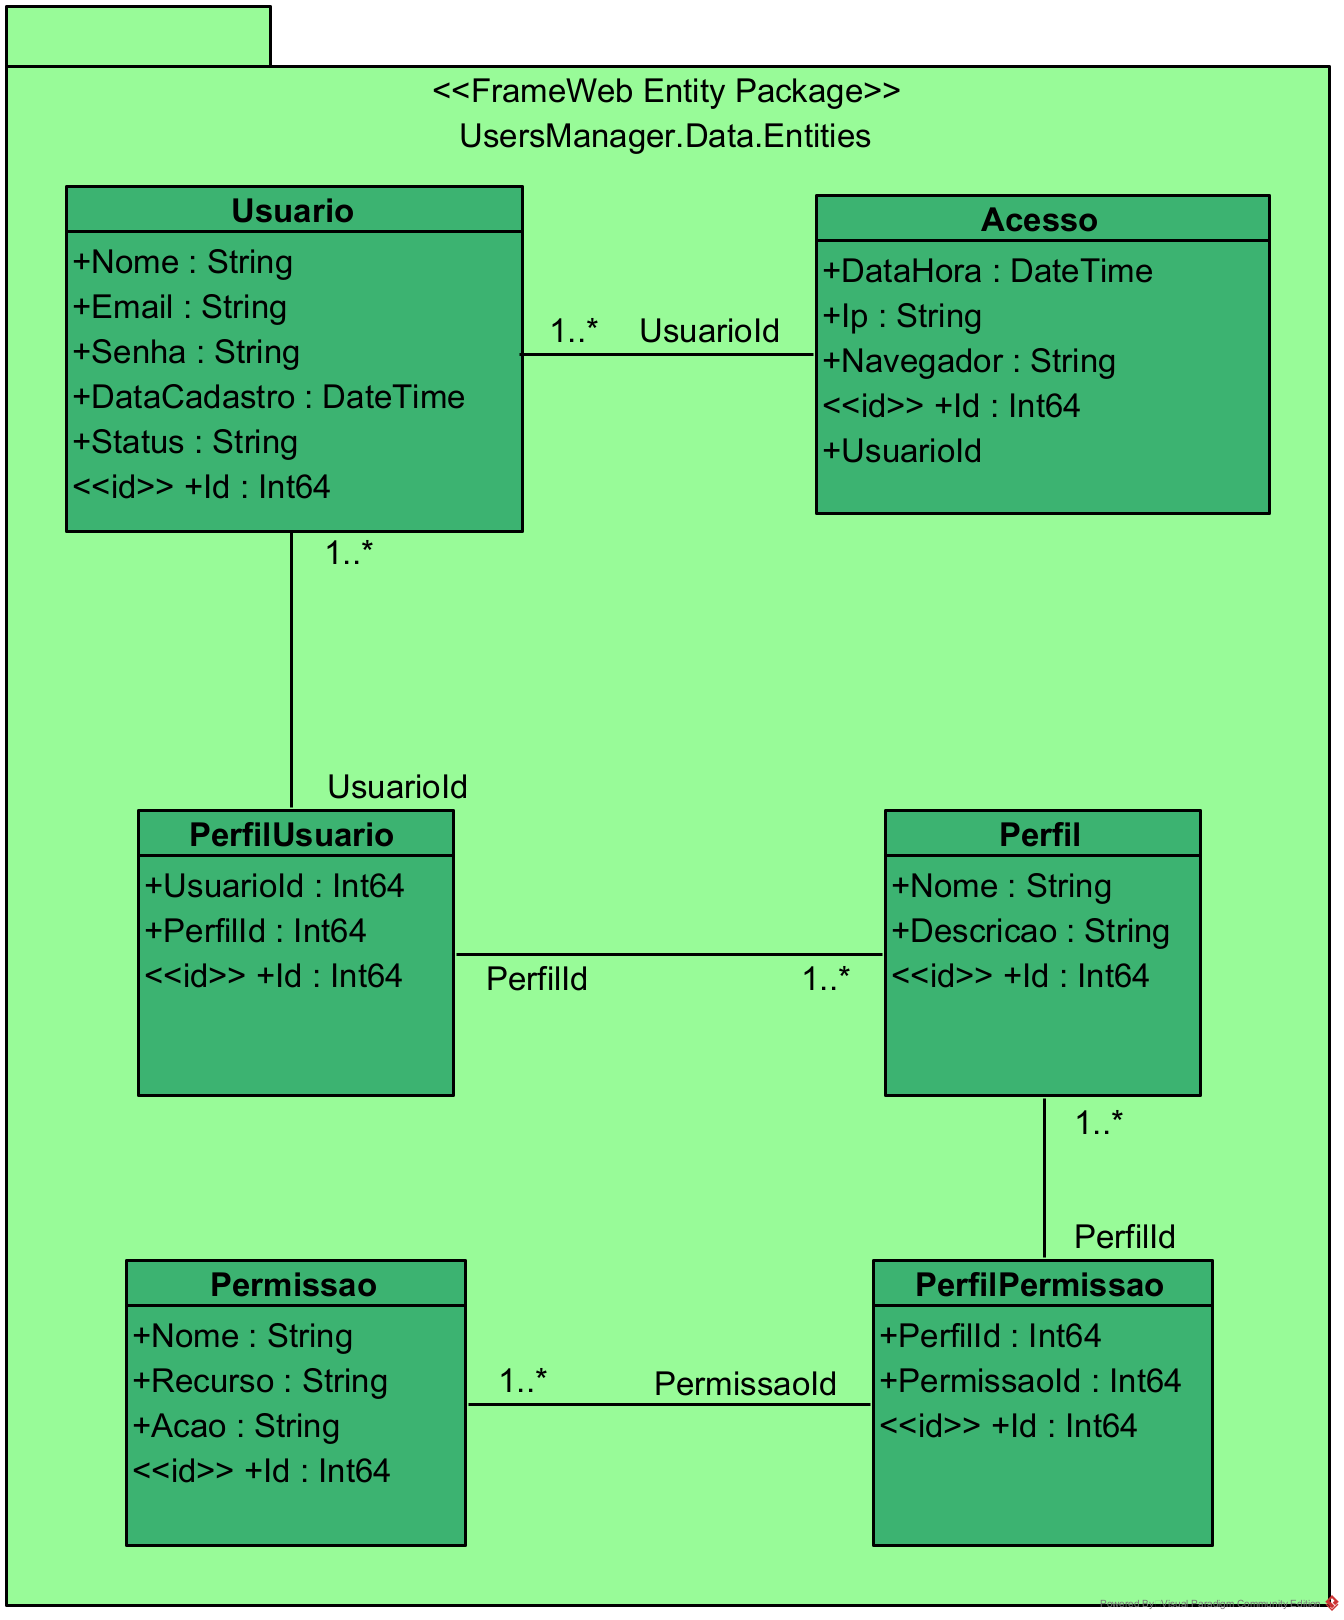
\includegraphics[width=0.95\textwidth]{figuras/Entidades Class Diagram.png}
	\caption{Modelo de Entidades adaptado para .NET}
	\label{fig:modelo-entidades}
\end{figure}

\begin{figure}[H]
	\centering
	\includegraphics[width=0.95\textwidth]{figuras/Aplicacao Class Diagram.png}
	\caption{Modelo de Aplicação adaptado para .NET}
	\label{fig:modelo-aplicacao}
\end{figure}

A principal adaptação aqui é a ausência de anotações específicas do Java (como \texttt{@Entity}, \texttt{@EJB}), substituídas por convenções e atributos do C\# e pelo uso de injeção de dependência nativa da plataforma.

\section{Camada de Acesso a Dados}
\label{sec-frameweb-dados}

A modelagem da camada de persistência também seguiu o modelo FrameWeb, representando os repositórios responsáveis por encapsular o acesso ao banco de dados. A principal diferença está no uso do \textbf{Entity Framework Core}, ao invés de JPA, e da \textbf{injeção de dependência} por meio do contêiner do ASP.NET.

\begin{figure}[H]
	\centering
	\includegraphics[width=0.9\textwidth]{figuras/Persistencia Class Diagram.png}
	\caption{Modelo de Persistência adaptado para .NET}
	\label{fig:modelo-persistencia}
\end{figure}

As interfaces e classes que implementam os repositórios foram modeladas conforme a abordagem recomendada para aplicações ASP.NET, respeitando a separação entre responsabilidades.

\section{Camada de Apresentação}
\label{sec-frameweb-apresentacao}

A modelagem da camada de apresentação também foi adaptada do modelo FrameWeb. Foram utilizados diagramas de navegação para representar os fluxos entre as páginas e os controladores, com base nas rotas configuradas no ASP.NET Core MVC.

\begin{figure}[H]
	\centering
	\includegraphics[width=0.9\textwidth]{figuras/Navegacao - Login.png}
	\caption{Navegação: Tela de Login}
	\label{fig:navegacao-login}
\end{figure}

\begin{figure}[H]
	\centering
	\includegraphics[width=0.9\textwidth]{figuras/Navegacao - Ver Dashboard.png}
	\caption{Navegação: Dashboard Principal}
	\label{fig:navegacao-dashboard}
\end{figure}

\begin{figure}[H]
	\centering
	\includegraphics[width=0.9\textwidth]{figuras/Navegacao - Edicao de Usuario.png}
	\caption{Navegação: Edição de Usuário}
	\label{fig:navegacao-edicao-usuario}
\end{figure}

\begin{figure}[H]
	\centering
	\includegraphics[width=0.9\textwidth]{figuras/Navegacao - Edicao de Perfil.png}
	\caption{Navegação: Edição de Perfil e Permissões}
	\label{fig:navegacao-edicao-perfil}
\end{figure}

Os controladores ASP.NET Core fazem o papel dos \textit{front controllers}, e os fluxos de navegação seguem a estrutura de rotas definida pelo framework.
